\documentclass[
  11pt,
  letterpaper,
   addpoints,
   %answers
  ]{exam}

\usepackage{../exercise-preamble}

\begin{document}

\noindent
\begin{minipage}{0.47\textwidth}

\includegraphics[width=\textwidth]{../fcfm_die}
\end{minipage}
\begin{minipage}{0.53\textwidth}
\begin{center} 
\large\textbf{Fundamentos de control de sistemas} (EL4111-1) \\
\large\textbf{Clase auxiliar 6} \\
\small Prof.~Roberto Cardenas Dobson\\
\small Prof.~Aux.~Osvaldo Jimenez - Erik Sáez\\
\small Ayudantes.~Simon Arenas- Juan Pablo Baez - Francisco Garces - Sofia Ibarra\\
\end{center}
\end{minipage}

\vspace{0.5cm}
\noindent
\vspace{.85cm}

\begin{questions}
%----------------------------------------------
    \question Considere el siguiente diagrama de control por lazos anidados, se pide:

    \begin{figure}[h!]
        \centering
        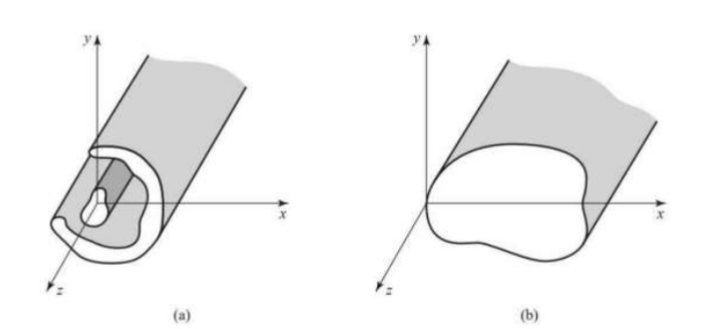
\includegraphics[width=0.8\textwidth]{Auxiliar_8_1} % Aquí va la imagen del diagrama
        \caption{Sistema de lazo de control discreto}
    \end{figure}
    
    \noindent \textbf{Indicación:} Realice sus cálculos aproximando al cuarto decimal. Para las secciones (a) y (b) considere $H(z) = 1$.
    
    \begin{enumerate}
        \item[(a)] Considerando una frecuencia de muestreo de 900 [rad/s] y mediante la transformada z exacta, demuestre que la planta discretizada del lazo externo es la siguiente (Incluya un retenedor de orden cero si es necesario): (10/50)
        \[
        G_p(z) = \frac{0.0124}{z - 0.7827}
        \]
        
        \item[(b)] Diseñe un controlador discreto para el lazo externo con cero error estacionario a entrada escalón, tal que sintonice un par de polos de lazo cerrado con amortiguamiento de $\xi = 0.707$ y una frecuencia natural de $w_n = 28$ [rad/s]. Ignore el lazo interno en este punto. (10/50)
        
        \item[(c)] Debido al envejecimiento del sistema de comunicaciones, se produce un retardo de transporte de 3 muestras en el lazo de retroalimentación $H(z)$. Dado que el controlador diseñado anteriormente ya está implementado en el sistema, se le pide a usted diseñar una malla de adelanto o atraso en cascada al controlador que permita que el sistema vuelva al punto de diseño anterior. Nuevamente, no considere el lazo interno. (15/50)
        
        \item[(d)] Ahora solo considere el lazo interno de la figura. Asumiendo un $K > 0$, encuentre el rango de ganancias de $K$ tal que el lazo interno sea estable. (10/50)
    
    \end{enumerate}
%----------------------------------------------
\begin{solution}
    \subsection*{Resolucion 1.1}
    Se busca obtener la planta discretizada del lazo externo, para esto se debe considerar la freuencia de muestreo es  $w_{s} = 900[rad/s]$ y por tanto el periodo de muestreo vendra dado por $T = \frac{2\pi}{w_{s}} \approx 0.007[s]$. Un aspecto importante a tener en consideracion es la ubicacion del muestreador, esto se observa en lo siguiente:
    \begin{center}
        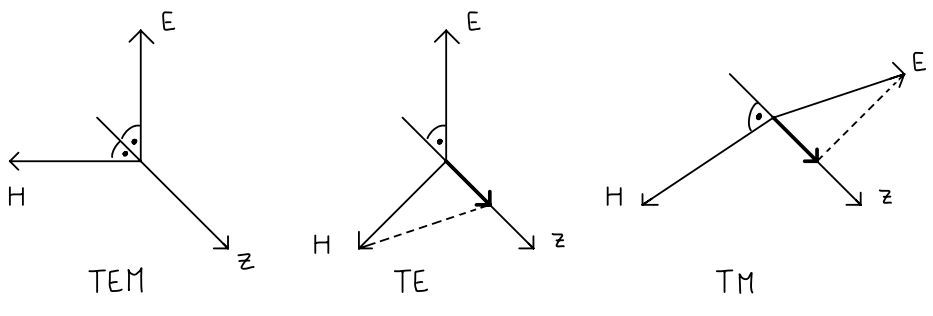
\includegraphics[width=0.6\textwidth]{Auxiliar_8_2}
        \captionof{figure}{Tipos de muestreo en una planta.}
    \end{center}
    Notamos que es importante analizar en que posicion se encuentra el muestreador, como el muestreado no se encuentra de manera explicita, podemos asumir el primer caso. Luego la planta discretizada vendra dada por:
    \begin{align}
        G_{p}(z) = Z\left< \left(\frac{1-e^{-sT_{s}}}{s}\right) \cdot \left( \frac{2}{s+35}\right)\right>
    \end{align}
    Donde el primer termino esta asociado a el ZOH (Retenedor de orden cero) Luego se aplica la transformada Z tal que:
    \begin{align}
        G_{p}(z) = \frac{z-1}{z}\cdot Z\left< \left( \frac{2}{s(s+35)}\right)\right>
    \end{align}
    Luego aplicando fracciones parciales se tiene que:
    \begin{align}
        \frac{2}{s(s+35)} &= \frac{A}{s} + \frac{B}{s+35}\\
        &= \frac{A(s+35) + Bs}{s(s+35)}
    \end{align}
    Con lo que se obtiene que:
    \begin{align}
        s(A+B) + 35A = 2\\
        A&= \frac{2}{35} & B&=\frac{-2}{35}
    \end{align}
    volviendo sobre la ecuacion anterior se tiene que:
    \begin{align}
        G_{p}(z) = \frac{z-1}{z}\cdot Z\left< \frac{2}{35}\left(\frac{1}{s} - \frac{1}{s+35}\right)\right>
    \end{align}
    Utilizando que :
    \begin{align}
        Z\left<\frac{1}{s+a} \right> = \frac{z}{z-e^{-aT_{S}}}
    \end{align}
    Se tendra finalmente que:
    \begin{align}
        G_{p}(z) = \frac{z-1}{z}\cdot \frac{2}{35}\left(\frac{z}{z-1} - \frac{z}{z-e^{-35\cdot 0.007}}\right)
    \end{align}
    Con lo que simplificando mediante TI, se obtiene que:
    \begin{align}
        G_{p}(z)= \frac{0.0124}{z-0.7827}
    \end{align}
    \subsection*{Resolucion 1.2}
    Dado que se busca sintonizar el lazo externo del contrador considerando que $\zeta = 0.707$ y $w_{n} = 28[rad/s]$ luego tenemos que evaluado en el punto de diseño en Z el cual viene dado:
    \begin{align}
        Z= e^{sT_{s}}
    \end{align}
    Donde tenemos que:
    \begin{align}
        s_{1,2}^{*} &= -\zeta w_{n} \pm jw_{n}\sqrt{1-\zeta^{2}}\\
    \end{align}
    Con lo que reemplazando los valores conocidos se tiene que:
    \begin{align}
        z= 0.8623 \pm j0.1203
    \end{align}
    De esta manera se tiene el puntoi de diseño, por lo que se propondra un controlador PI tal que:
    \begin{align}
        G_{PI}(z) = K\frac{(z-a)}{(z-1)}
    \end{align}
    Donde debemos recordar que (z-1) produce cero error a estado estacionario. Tenemos que el LGR en el dominio Z vendra dado por:
    \begin{center}
        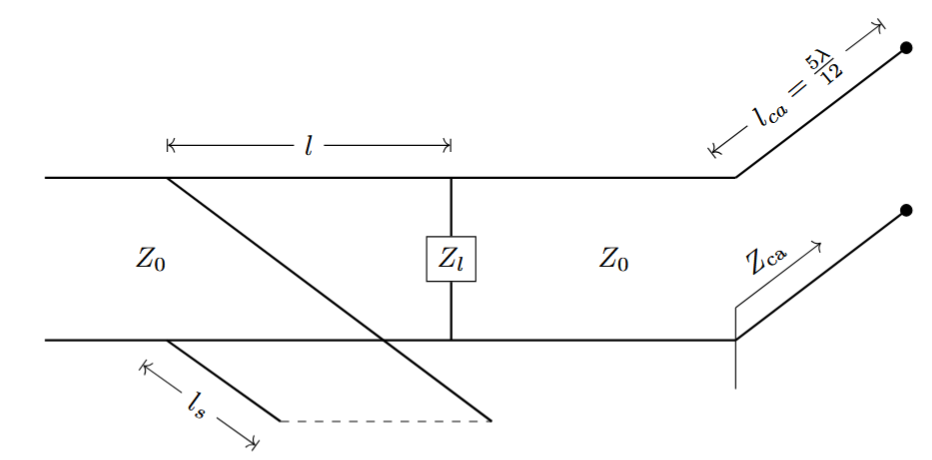
\includegraphics[width=0.6\textwidth]{Auxiliar_8_5}
        \captionof{figure}{LGR de la planta.}
    \end{center}
    De tal manera que por condicion de angulo se tendra que:
    \begin{align}
        \theta_{1} &= 180^{\circ} - \tan^{-1}\left(\frac{0.1203}{1-0.8623}\right) = 138.9^{\circ}\\
        \theta_{0.7827} & = \tan^{-1}\left(\frac{0.1203}{0.8623-0.7827}\right) = 56.51^{\circ}
    \end{align}
    Con lo que tenemos lo siguiente:
    \begin{align}
        \theta_{0.7827} + \theta_{1} - \theta_{a} = 180^{\circ}\\
        \theta_{a} = 15.41^{\circ}
    \end{align}
    Luego tendremos que a se ubica a la izquierda del punto de diseño, es por esto que:
    \begin{align}
        \theta_{a} = \tan^{-1}\left(\frac{0.1203}{0.8623-a}\right) = 15.41^{\circ}
    \end{align}
    Con lo que $a=0.4259$, con lo que la ganancia sera:
    \begin{align}
        K = \left| \frac{1}{\frac{0.0124}{z-0.7827} \frac{z-0.4259}{z-1}}\right|_{z = 0.8623 + j \, 0.1203} = 4.699
    \end{align}
    Con lo que se obtiene el controlador.
    \subsection*{Resolucion 1.3}
    Dado que se busca corregir el retardo de transporte de 3 muestras, se debe considerar un controlador de adelanto o atraso, pero no se puede modificar el controlador realizado previamente. Por lo qu ela idea es hacer una malla del siguiente tipo:
    \begin{align}
        G_{c2}(z) = K_{c2}\frac{z-b}{z-0.4259}
    \end{align}
    El denominador permite cancelar el cero del controlador anterior, de esta manera el nuevo LGR considerando las 3 muestras de retraso ademas de el nuevo controlador:
    \begin{center}
        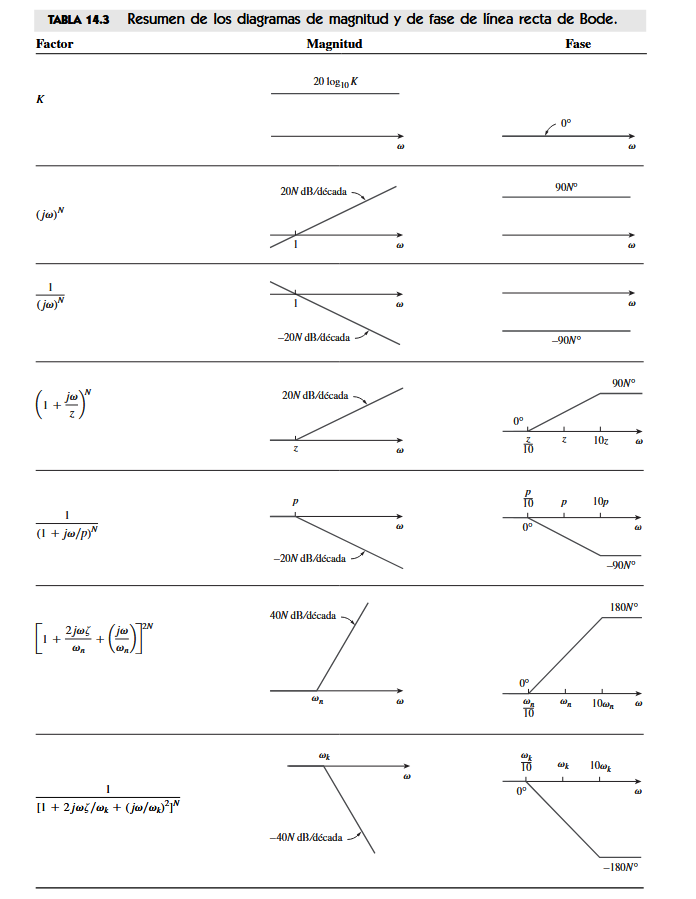
\includegraphics[width=0.6\textwidth]{Auxiliar_8_6}
        \captionof{figure}{LGR de la planta considerando muestreo.}
    \end{center}
    Con lo que tenemos practicamente los mismo angulos de antes, pero con la diferencia del retardo es por esto que:
    \begin{align}
        \theta_{r} = atan\left(\frac{0.1203}{0.8623}\right) = 7.942^{\circ}
    \end{align}
    Con lo que se tiene que la condicion de angulo sera:
    \begin{align}
        (\theta_{0.7827} + \theta_{1} + 3 \theta_{r}) - \theta_{b} = 180^{\circ}
    \end{align}
    Se tiene que:
    \begin{align}
        \theta_{b} = 39.24^{\circ}
    \end{align}
    De esta manera tenemos que $b = 0.715$ con lo que la ganancia sera:
    \begin{align}
        K = \left| \frac{1}{\frac{0.0124}{z-0.7827}\cdot 4.699 \cdot \frac{z-0.4259}{z-1} \cdot \frac{1}{z^{3}} \cdot \frac{z-0.715}{z-0.4259}}\right|_{z = 0.8623 + j \, 0.1203} = 1.571
    \end{align}
    De esta manera tenemos que:
    \begin{align}
        G_{c2}(z) = 1.571\frac{z-0.715}{z-0.4259}
    \end{align}
    con lo que ambos controladores resultaran en:
    \begin{align}
        G'_{c}(z) &= 4.699 \cdot 1.571 \cdot \frac{z-0.4259}{z-1} \cdot \frac{z-0.715}{z-0.4259}
        &= 7.382 \cdot \frac{z- 0.715}{z-1}
    \end{align}
    Otra forma de resolver el problema podrias ser proponiendo un controlador de la forma:
    \begin{align}
        G_{c2}(z) = K_{c2}\frac{z-0.7287}{z-B}
    \end{align}
    \subsection*{Resolucion 1.4}
    Se busca analizar el rango de valores de $K > 0$ tal que lazo interno sea estable. Tenemos que el lazo interno es de la forma:
    \begin{align}
        G_{int}(z) = \frac{K}{z(z-0.75)}
    \end{align}
    Notamos que es un LGR conocido, por lo tanto se tiene que:
    \begin{center}
        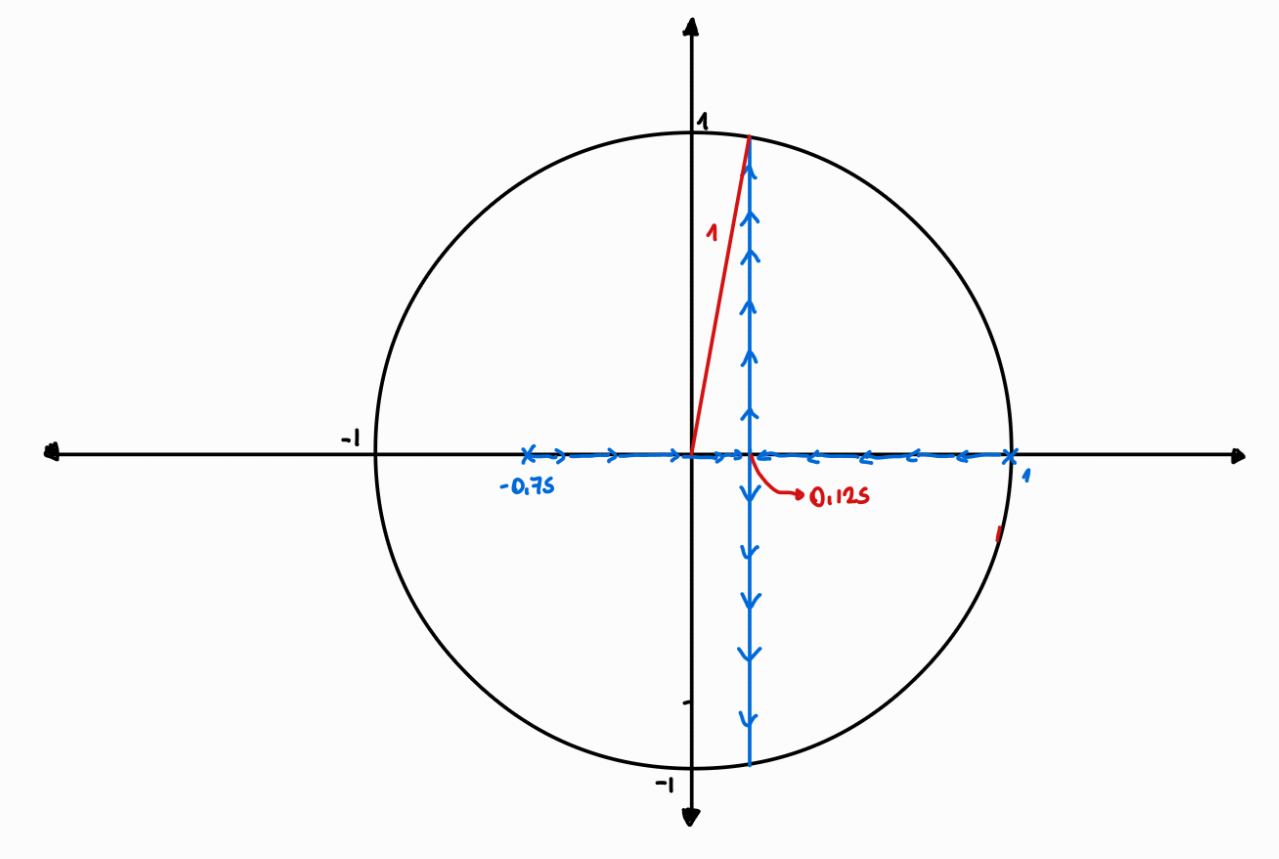
\includegraphics[width=0.55\textwidth]{Auxiliar_8_8}
        \captionof{figure}{LGR de la planta.}
    \end{center}
    Sabemos que el punto de salida del LGR vendra dado por el punto medio, es decir:
    \begin{align}
        a= \frac{1+0.75}{2} = 0.875
    \end{align}
    Por lo que las asintotas se ubicaran en $1-a = 1-0.875 = 0.125$. Luego tenemos que:
    \begin{center}
        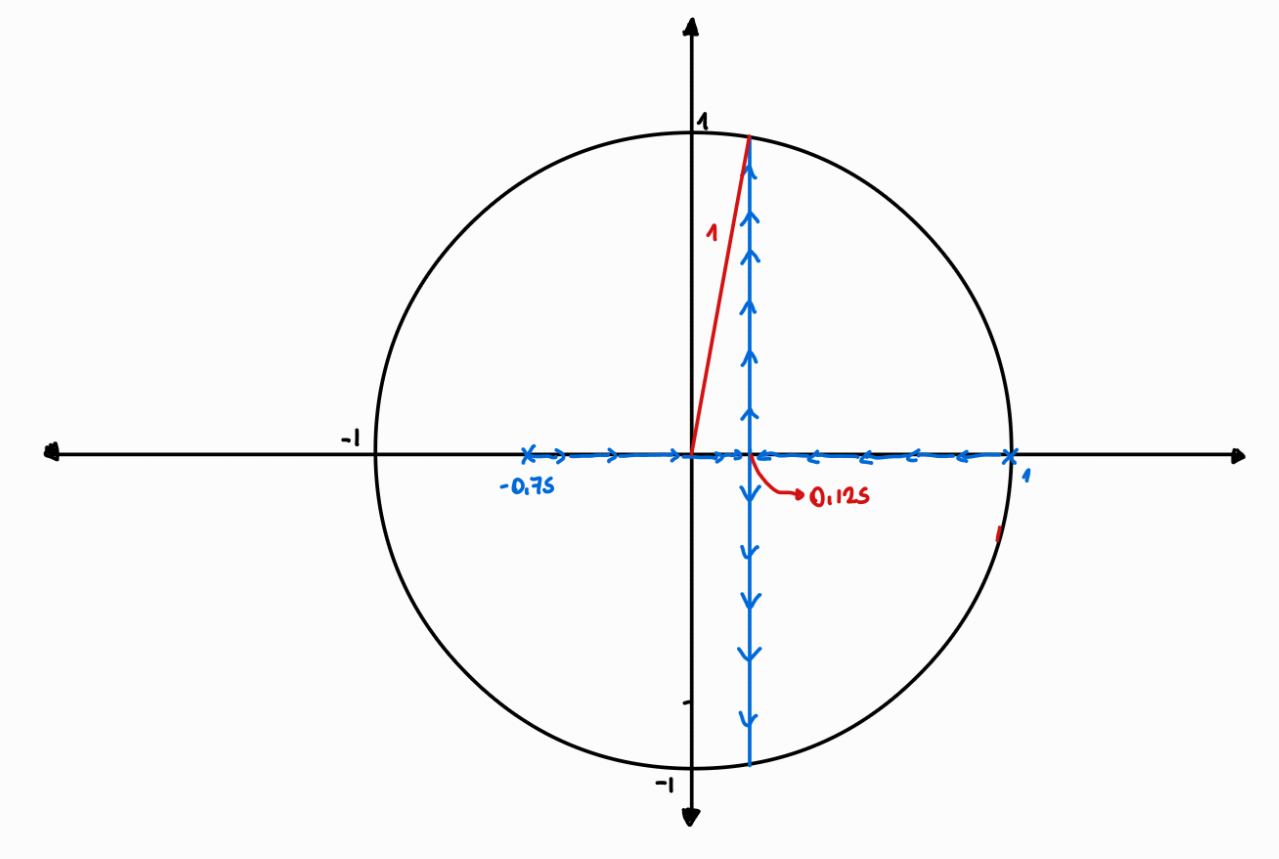
\includegraphics[width=0.55\textwidth]{Auxiliar_8_8}
        \captionof{figure}{LGR de la planta.}
    \end{center}
    Tenemos que mediante Pitagoras es directo despejar el valor de la altura, es decir que:
    \begin{align}
        \sqrt{0.125^{2} + Y^{2}} &= 1\\
        Y &= 0.992
    \end{align}
    Se tendra que el valor de Z critico correspondera a:
    \begin{align}
        z^{*} = 0.125 + j0.992
    \end{align}
    Con lo que ahora es posible obtener el valor de la ganancia critica tal que:
    \begin{align}
        K_{c} = \left| \frac{1}{\frac{1}{(z-1)(z+0.75)}}\right|_{z = 0.125 + j \, 0.992} = 1.75
    \end{align}
    Con lo que se tendra que para un $k< 1.75$ el sistema sera estable.
    \subsection*{Resolucion 1.5}
    Termianr de AGREGAR
\end{solution}
%----------------------------------------------
    \question 
    \begin{enumerate}
        \item[(a)] Demuestre matemáticamente y haciendo aproximaciones adecuadas, que un retenedor de orden cero produce un retardo de aproximadamente media muestra.
        
        \item[(b)] Dado el siguiente sistema a lazo abierto en \( z \) con un tiempo de muestreo \( T_s = 0.1 \):
        \[
        \frac{z + 1}{z - 0.6}
        \tag{1}
        \]
        Utilizando LGR, encuentre un controlador proporcional que a lazo cerrado permita obtener un coeficiente de amortiguamiento de \( \xi = 0.532 \). ¿Cuál sería la frecuencia natural obtenida para este punto?
    \end{enumerate}
%----------------------------------------------
\begin{solution}
\subsection*{Resolucion 2.1}
Se busca demostrar que un retenedor de orden cero produce un retardo de aproximadamente media muestra, para esto se debe considerar que un retenedor de orden cero vendra dado por:
\begin{align}
    ZOH(s)= \frac{1-e^{-Ts}}{s}
\end{align}
Luego aplicando la aproximacion de Taylor tenemos que: $e^{-sT}= 1 - sT + \frac{(sT)^{2}}{2!} - \frac{(sT)^{3}}{3!} \ldots $, con lo que tenemos que reemplazando hasta el segundo orden:
\begin{align}
    ZOH(s) &= \frac{1-(1-sT + \frac{(sT)^{2}}{2!})}{s}\\
    &= \frac{sT - \frac{(sT)^{2}}{2}}{s}\\
    &= T - \frac{T^{2}}{2}s\\
    &= T(1- \frac{T}{2}s)\\
    &\approx T(e^{-\frac{T}{2}s})
\end{align}
Con lo que se observa que efectivamente el retenedor de orden cero produce un retardo de aproximadamente media muestra.
\subsection*{Resolucion 2.2}
Tenemos que el sistema a lazo abierto vendra dado por:
\begin{align}
    G_{p}(z) = \frac{z+1}{z-0.6}
\end{align}
Luego Tenemos que el LGR vendra dado por:
\begin{center}
    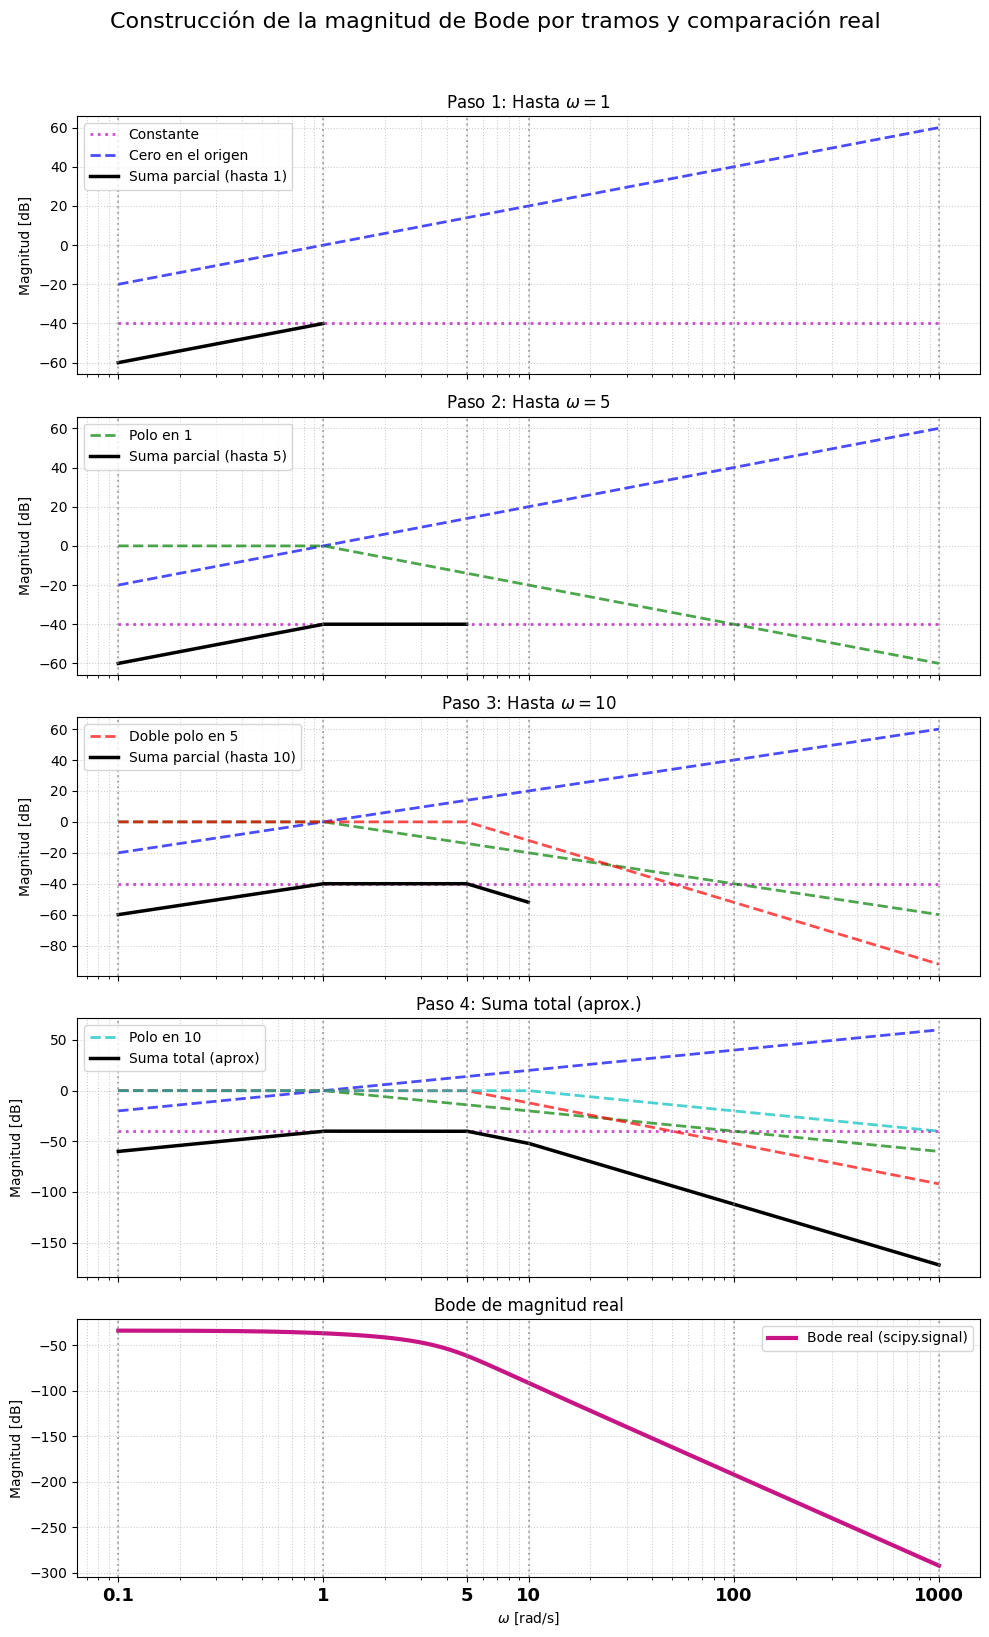
\includegraphics[width=0.55\textwidth]{Auxiliar_8_9}
    \captionof{figure}{LGR de la planta.}
\end{center}
\begin{align}
    Z= e^{sT_{s}}
\end{align}
Donde tenemos que $s=\frac{1}{T}\ln(z)$ donde podemos definir $z=re^{j\theta}$, luego como el LGR se encuentra unicamente en el eje real, tendremos que $\theta = \pi$, por lo que se tiene que:
\begin{align}
    s = \frac{1}{T}( \ln(r) + j \pi) 
\end{align}
Sabemos que de manera general 
\begin{align}
    \theta = atan\left(\frac{Im(s)}{Re(s)}\right)
\end{align}
y como tenemos ademas que $\zeta = cos(\theta)$ se tendra que:
\begin{align}
    \tan(arcos(\zeta)) = \frac{\pi}{\ln(r)}
\end{align}
donde $r=0.1389$ por lo que se tendra que z=0.-1389, con lo que se tiene que la ganancia vendra dada por:
\begin{align}
    K = \left| \frac{1}{\frac{z+1}{z-0.6}}\right|_{z=0.1389} = 0.858
\end{align}
Con lo que finalmente se tendra que la frecuencia buscada sera:
\begin{align}
    w_{n} = \frac{1}{T} \sqrt{\ln(0.1389)^{2}+\pi^{2}}= 37.1 [rad/s]
\end{align}
Finalmente se obtiene la frecuencia.
\end{solution}
%----------------------------------------------
\question Se desea diseñar una estrategia de control digital para poder controlar la velocidad en un motor síncrono. El diagrama de bloques del sistema en lazo cerrado es el que se muestra en la siguiente página (Fig. 2).
\[
G(s) = \frac{10}{(s + 1)(s + 5)}
\]
\begin{figure}[h!]
    \centering
    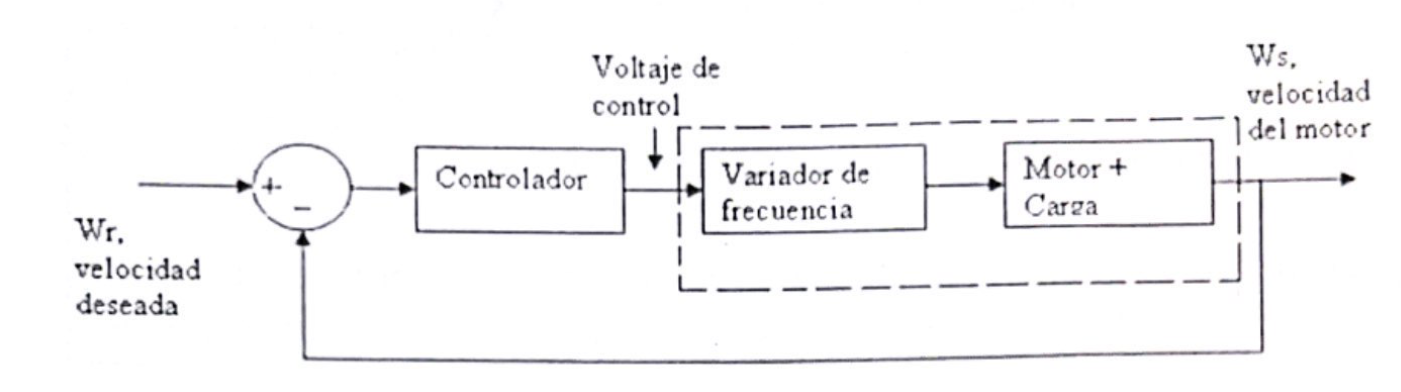
\includegraphics[width=0.8\textwidth]{Auxiliar_8_3}
    \caption{Diagrama de bloques del sistema en lazo cerrado.}
\end{figure}
Se pide:
\begin{itemize}
    \item[a)] Discretizar el sistema utilizando la transformada \( z \) exacta y considerando un tiempo de muestreo de \( T = 0.2 \) seg. Si es necesario, inserte un retenedor de orden cero antes del actuador.
    \item[b)] Dibuje el LGR en el plano \( z \), identifique las asíntotas y encuentre los posibles puntos de arranque y llegada en el eje real.
    \item[c)] Diseñe, utilizando los criterios del módulo y ángulo del LGR, un sistema de control que entregue cero error en estado estacionario a entrada escalón, un sobrepaso de 16\% y tiempo de establecimiento de \( \approx 3 \) seg.
\end{itemize}
%-----------------------------------------------
\begin{solution}
\subsection*{Resolucion 3.1}
Se busca discretizar el sistema, para esto se debe considerar que el sistema en lazo cerrado vendra dado por:
\begin{align}
    G_{p}(s) = \frac{10}{(s+1)(s+5)}
\end{align}
Con lo que discretizando el sistema se tiene que:
\begin{align}
    G_{p}(z) = Z\left< \frac{1-e^{-sT_{s}}}{s}\right> \cdot Z\left< \frac{10}{(s+1)(s+5)}\right>
\end{align}
Similar a la primera pregunta tenemos que:
\begin{align}
    G_{p}(z) = \frac{z-1}{z}\cdot Z\left< \frac{10}{s(s+1)(s+5)}\right>
\end{align}
Aplicando fracciones parciales tenemos que:
\begin{align}
    \frac{10}{s(s+1)(s+5)} &= \frac{A}{s} + \frac{B}{s+1} + \frac{C}{s+5}\\
    &= \frac{A(s+1)(s+5) + B(s)(s+5) + C(s)(s+1)}{s(s+1)(s+5)}\\
    &= \frac{(A+B+C)s^{2} + (6A + 5B + C)s + 5A}{s(s+1)(s+5)}
\end{align}
Luego el sistema de ecuaciones correspondera a:
\begin{align}
    A+B+C &= 0\\
    6A + 5B + C &= 10\\
    5A &= 10
\end{align}
Dando como resultado que $A=2$, $B=-\frac{5}{2}$ y $C=\frac{1}{2}$, con lo que se tiene que:
\begin{align}
    G_{p}(z) = \frac{z-1}{z}\cdot \left( Z\left< \frac{2}{s} \right> + Z\left< \frac{(-5/2)}{s+1}\right> + Z\left< \frac{1/2}{(s+5)} \right>  \right)
\end{align}
Con lo que finalmente se obtiene que:
\begin{align}
    G_{p}(z) = \frac{z-1}{z} \cdot \left( \frac{2}{z-1} + \frac{(-5/2)z}{z-e^{-0.2}} + \frac{(1/2)z}{z-e^{-5\cdot 0.2}}\right)
\end{align}
Luego tenemos que mediante TI se obtiene que:
\begin{center}
    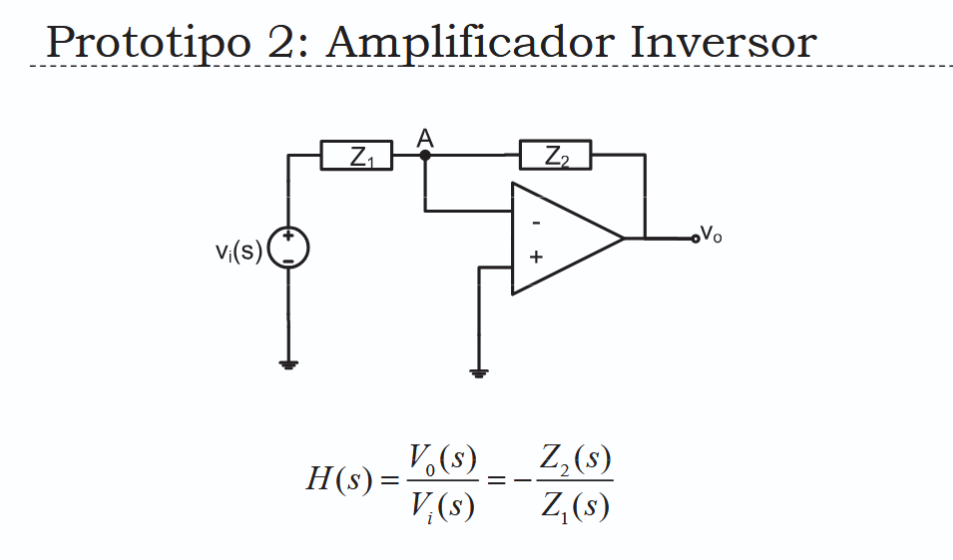
\includegraphics[width=0.5\textwidth]{Auxiliar_8_4}
    \captionof{figure}{Valor en TI}
\end{center}
Tenmos que el termino en rojo es bastante cercano a 0, por lo que se puede despreciar, con lo que se obtiene que:
\begin{align}
    G_{p}(z)= \frac{0.1371 (z+0.6714)}{(z-8187)(z-0.3679)}
\end{align}
Con lo que se obtiene la forma de la planta exacta discretizada.
\subsection*{Resolucion 3.2}
Se busca obtener el LGR en el plano Z, para lo que se pide identificar las asintotas y los posibles puntos de arranque y llegada en el eje real.

Se tiene que los puntos de partida mirando la planta son seran $p_{1} = 0.8187$ y $p_{2} = 0.3679$. Luego el numero de asintotas correspondera sera $\#p - \#z = 2-1 =1 $ por lo que las asintotas sera:
\begin{align}
    \theta_{a} = \frac{(2n+1)\pi}{N^{\circ} Asintota} = \frac{(2\cdot 0 +1)\pi}{N^{\circ} Asintota} = \pi
\end{align}
Es decir que tenemos una sola asintota. Luego por enunciado se busca obtener los valores de corte en el eje real , por lo tanto:
\begin{align}
    \frac{\partial K}{\partial z} = 0
\end{align} 
De la ecuacion caracteristica se despeja el valor de k tal que:
\begin{align}
    K=  -\frac{(z-0.8187)(z-0.3679)}{(z+0.6714)}
\end{align}
Derivamos e igualamos a 0 obteniendo que:
\begin{align}
    z_{1} = -1.916
    z_{2} = 0.571
\end{align}
Luego se observa que ambos puntos deben pertenecer al LGR, por lo que no podemos descartar ninguno de los dos puntos, esto se observa en:
%- AGREGAR LGR EN Z -%
Por lo tanto tenemos finalmente que el LGR de la planta en el plano Z vendra dado por:
%0- AGREGAR LGR EN Z -%
\subsection*{Resolucion 3.3}
Se busca diseñar un sistema de control que entregue cero error en estado estacionario a entrada escalon, un sobrepaso de 16\% y tiempo de establecimiento de \( \approx 3 \) seg. Por lo tanto:
\begin{align*}
    16 = 100 \cdot e^{-\frac{\xi \pi}{\sqrt{1-\xi^{2}}}}
\end{align*}
Dando como resultado que \( \xi = 0.5039 \). Luego se tiene que para el tiempo de establecimiento:
\begin{align*}
    T_{s} = \frac{4}{\xi w_{n}} = 3
\end{align*}
Considernado lo obtenido anteriormente, tenemos que:
\begin{align*}
    w_{n} = \frac{4}{3 \cdot 0.5039} = 2.65 [rad/s]
\end{align*}
En base a esto, es posible obtener luego los puntos de diseños dado por:
\begin{align*}
    z=e^{sT} = e^{-\xi w_{n}T} \cdot e^{jw_{n}\sqrt{1-\xi^{2}}T}
\end{align*}
Reemplazando el valor de $w_{n}$ y $\xi$ se tendra:
\begin{align*}
    z= 0.6873 \pm j0.338
\end{align*}
Para la sintonizacion podemos haer uso de un controlador PI: 
\begin{align}
    G_{PI}(z) = K\frac{z-a}{z-1}
\end{align}
Luego el LGR  en el dominio Z vendra dado por:
%%- AGREGAR LGR EN Z -%%
\begin{align}
    \theta_{z}&= atan\left(\frac{0.338}{0.6714+0.6873}\right) = 13.97^{\circ}\\
    \theta_{p1}& = atan\left(\frac{0.338}{0.6873-0.3679}\right) = 46.62^{\circ}\\
    \theta_{p2}& = 180^{\circ} - atan\left(\frac{0.338}{0.8187-0.6873}\right) = 111.2^{\circ}\\
    \theta_{PI}&= 180 - atan\left(\frac{0.338}{1-0.6873}\right) = 132.8^{\circ} 
\end{align}
Con lo que considerando un angulo $\theta_{a}$ asociado al cero del controlador se tiene que:
\begin{align*}
    \theta_{a} = 96.65^{\circ}
\end{align*}
Dando asi un $a =0.7267$ y con esto es posible el obtener la ganancia dada por:
\begin{align}
    K = \left| \frac{1}{\frac{0.1371(z+0.6714)(z-0.7265)}{(z-0.7187)(z-0.3679)(z-1)}}\right|_{z=0.6873 + j0.338} = 1.189
\end{align}
Dando como resultado un controlador de la forma:
\begin{align}
    G_{PI}(z) = 1.189\frac{z-0.7265}{z-1}
\end{align}
%----------------------------------------------
\end{solution}
\end{questions}
\newpage
%%%%%%%%%%%%%%%%%%%%%%%%%%%

\end{document}